\documentclass[10pt, aspectratio=169]{beamer}

% Hỗ trợ tiếng Việt với XeLaTeX
\usepackage{polyglossia}
\setdefaultlanguage{vietnamese}
\usepackage{fontspec}
\setmainfont{Times New Roman}
\setsansfont{Arial}
\setmonofont{Courier New}

\usepackage{tikz}
\usetikzlibrary{shapes.geometric, arrows.meta, positioning, fit, calc, backgrounds}

\usepackage{amsmath}
\usepackage{graphicx}
\usepackage{tabularx}
\usepackage{booktabs}

% Cấu hình màu sắc NutriTrack
\definecolor{NutriDark}{HTML}{003139}
\definecolor{NutriGreen}{HTML}{5FE089}
\definecolor{NutriLightGray}{HTML}{F8F9FA}

\setbeamercolor{palette primary}{bg=NutriDark,fg=white}
\setbeamercolor{palette secondary}{bg=NutriGreen,fg=NutriDark}
\setbeamercolor{structure}{fg=NutriDark}
\setbeamercolor{frametitle}{bg=NutriDark,fg=white}
\setbeamercolor{background canvas}{bg=NutriLightGray}
\setbeamercolor{normal text}{fg=black!85}
\setbeamercolor{itemize item}{fg=NutriGreen}
\setbeamercolor{itemize subitem}{fg=NutriDark}

% Cấu hình template
\setbeamertemplate{navigation symbols}{}
\setbeamertemplate{footline}[frame number]
\setbeamertemplate{itemize item}{\tikz\fill[NutriGreen] (0,0) circle (2pt);}
\setbeamertemplate{itemize subitem}{\tikz\fill[NutriDark] (0,0) circle (1.5pt);}

% Component tái sử dụng
\newcommand{\modulelabel}[1]{\tikz[baseline=(char.base)]\node[anchor=text, rectangle, draw=NutriDark, fill=NutriDark!10, rounded corners=2pt, inner sep=3pt, text=NutriDark, font=\bfseries] (char) {#1};}
\newcommand{\highlightblue}[1]{\textcolor{NutriDark}{\textbf{#1}}}
\newcommand{\highlightgreen}[1]{\textcolor{NutriGreen!80!black}{\textbf{#1}}}

% Thông tin tiêu đề (dùng cho các frame khác nếu cần)
\title{\textbf{HỆ THỐNG QUẢN LÝ DINH DƯỠNG CÁ NHÂN HÓA}}
\subtitle{Personalized Nutrition Management System}
\author{\textbf{Sinh viên: Nguyễn Văn Khánh}\\ MSSV: 0241967 \quad Lớp: 67CS2 \\ \vspace{0.3cm} \small GVHD: TS. Phạm Hồng Phong}
\institute{Trường Đại học Xây dựng Hà Nội \\ Ngành Công nghệ thông tin - Chuyên ngành Khoa học máy tính}
\date{Năm 2026}

\begin{document}

% Thời lượng dự kiến: 20-30 giây
\begin{frame}[plain]
\begin{tikzpicture}[remember picture, overlay]

    % === PANEL TRÁI: NỀN TỐI (58% chiều rộng) ===
    \fill[NutriDark] (current page.south west)
        rectangle ([xshift=0.58\paperwidth]current page.south west |- current page.north west);

    % Vòng tròn trang trí góc trên trái
    \draw[NutriGreen, line width=4pt, opacity=0.18]
        ([xshift=-0.6cm, yshift=0.6cm]current page.north west) circle (1.8cm);
    \draw[NutriGreen, line width=1.5pt, opacity=0.10]
        ([xshift=-0.6cm, yshift=0.6cm]current page.north west) circle (2.8cm);

    % Vòng tròn trang trí góc dưới trái
    \fill[NutriGreen, opacity=0.07]
        ([xshift=1.8cm, yshift=-0.3cm]current page.south west) circle (2.2cm);
    \draw[NutriGreen, line width=2pt, opacity=0.18]
        ([xshift=1.8cm, yshift=-0.3cm]current page.south west) circle (2.2cm);

    % Thanh accent dọc màu xanh lá
    \fill[NutriGreen]
        ([xshift=0.85cm, yshift=3.2cm]current page.west)
        rectangle ([xshift=1.15cm, yshift=6.2cm]current page.west);

    % Tiêu đề đề tài (3 dòng, chữ lớn, bold, trắng)
    \node[text=white, font=\bfseries, text width=7.6cm, align=left, anchor=west]
        at ([xshift=1.6cm, yshift=1.3cm]current page.west) {
        {\fontsize{14.5}{20}\selectfont HỆ THỐNG QUẢN LÝ}\\[5pt]
        {\fontsize{14.5}{20}\selectfont DINH DƯỠNG}\\[5pt]
        {\fontsize{14.5}{20}\selectfont CÁ NHÂN HÓA}
    };

    % Subtitle (chữ nghiêng màu xanh lá nhạt)
    \node[text=NutriGreen!75, font=\itshape\small, text width=7.6cm, align=left, anchor=west]
        at ([xshift=1.6cm, yshift=-0.65cm]current page.west) {
        Personalized Nutrition Management System
    };

    % Nhãn nhỏ phía dưới trái
    \node[text=white!40, font=\scriptsize, align=left, anchor=west]
        at ([xshift=1.6cm, yshift=-1.65cm]current page.west) {
        Đồ án tốt nghiệp $\cdot$ Năm 2026
    };

    % === PANEL PHẢI: NỀN SÁNG (42% còn lại) ===
    % Logo trường
    \node[anchor=center]
        at ([xshift=0.79\paperwidth, yshift=0.74\paperheight]current page.south west) {
        
\includegraphics[height=1.9cm]{images/LOGO_DHXD.png}
    };

    % Tên trường
    \node[text=NutriDark, font=\small\bfseries, text width=5.6cm, align=center, anchor=center]
        at ([xshift=0.79\paperwidth, yshift=0.585\paperheight]current page.south west) {
        Trường Đại học Xây dựng Hà Nội
    };

    % Đường kẻ accent ngang
    \fill[NutriGreen]
        ([xshift=0.625\paperwidth, yshift=0.495\paperheight]current page.south west)
        rectangle ([xshift=0.955\paperwidth, yshift=0.508\paperheight]current page.south west);

    % Thông tin sinh viên
    \node[text=NutriDark!85, font=\small, text width=5.6cm, align=center, anchor=center]
        at ([xshift=0.79\paperwidth, yshift=0.385\paperheight]current page.south west) {
        {\bfseries Sinh viên: Nguyễn Văn Khánh}\\[5pt]
        MSSV: 0241967 \quad Lớp: 67CS2
    };

    % Giảng viên hướng dẫn
    \node[text=NutriDark!70, font=\small, text width=5.6cm, align=center, anchor=center]
        at ([xshift=0.79\paperwidth, yshift=0.255\paperheight]current page.south west) {
        {\bfseries GVHD:} TS. Phạm Hồng Phong
    };

    % Ngành học
    \node[text=NutriDark!50, font=\scriptsize, text width=5.6cm, align=center, anchor=center]
        at ([xshift=0.79\paperwidth, yshift=0.13\paperheight]current page.south west) {
        Ngành CNTT -- Chuyên ngành Khoa học máy tính
    };

\end{tikzpicture}
\end{frame}

% Thời lượng dự kiến: 50 giây
\begin{frame}{Đặt vấn đề}
    \begin{itemize}
        \setlength{\itemsep}{10pt}
        \item Người dùng cần theo dõi nhiều loại dữ liệu: ăn uống, năng lượng, cân nặng, nước và luyện tập.
        \item Việc ghi chép và tổng hợp thủ công tốn thời gian, phân tán.
        \item Giá trị TDEE ước tính từ công thức tĩnh có thể chưa phản ánh đầy đủ mức tiêu hao năng lượng thực tế của từng người theo thời gian.
        \item \highlightblue{Yêu cầu:} Một hệ thống thống nhất để theo dõi, phân tích và hỗ trợ điều chỉnh chế độ dinh dưỡng cá nhân hóa.
    \end{itemize}

    \begin{center}
    \begin{tikzpicture}[node distance=1.2cm, >=Stealth, 
        box/.style={rectangle, draw=NutriDark, fill=white, rounded corners, minimum height=0.8cm, text centered, font=\small},
        arrow/.style={->, thick, NutriDark}]
        
        \node[box] (data) {Dữ liệu phân tán};
        \node[box, right=of data] (track) {Khó theo dõi};
        \node[box, right=of track] (eval) {Khó đánh giá};
        \node[box, fill=NutriGreen!20, right=of eval] (sys) {\textbf{Cần hệ thống cá nhân hóa}};
        
        \draw[arrow] (data) -- (track);
        \draw[arrow] (track) -- (eval);
        \draw[arrow] (eval) -- (sys);
    \end{tikzpicture}
    \end{center}
\end{frame}

% Thời lượng dự kiến: 50 giây
\begin{frame}{Mục tiêu và phạm vi}
    \begin{columns}[T]
        \begin{column}{0.48\textwidth}
            \modulelabel{Mục tiêu hệ thống}
            \vspace{0.3cm}
            \begin{itemize}
                \item Xây dựng hệ thống web quản lý dinh dưỡng cá nhân.
                \item Theo dõi nhật ký ăn uống và các chỉ số cơ thể.
                \item Tính toán nhu cầu năng lượng và dinh dưỡng.
                \item Phân tích dữ liệu theo thời gian.
                \item Hỗ trợ lập kế hoạch bữa ăn và nhập liệu thực phẩm bằng mã vạch, hình ảnh nhãn dinh dưỡng.
            \end{itemize}
        \end{column}
        
        \begin{column}{0.48\textwidth}
            \modulelabel{Phạm vi ứng dụng}
            \vspace{0.3cm}
            \begin{itemize}
                \item Hồ sơ và mục tiêu cá nhân.
                \item Nhật ký dinh dưỡng.
                \item Cân nặng, lượng nước, và luyện tập.
                \item Dashboard và báo cáo PDF theo tuần/tháng.
                \item Lập kế hoạch bữa ăn (Meal Planner).
                \item Quét thông tin sản phẩm (Scanner).
            \end{itemize}
        \end{column}
    \end{columns}
\end{frame}

% Thời lượng dự kiến: 1 phút
\begin{frame}{Kiến trúc tổng thể của hệ thống}
    \begin{center}
    \begin{tikzpicture}[>=Stealth, node distance=0.6cm and 0.4cm,
        layer/.style={rectangle, draw=NutriDark, fill=white, rounded corners, text centered, minimum width=2.5cm, minimum height=0.6cm, font=\footnotesize},
        arrow/.style={->, thick, NutriDark}]
        
        \node[layer, fill=NutriGreen!20] (client) {\textbf{Người dùng}};
        \node[layer, below=of client] (react) {React SPA};
        \node[layer, below=of react] (api) {RESTful API};
        
        \node[layer, below left=1cm and -1cm of api] (controller) {Controller};
        \node[layer, right=of controller] (service) {Service};
        \node[layer, right=of service] (model) {Sequelize Model};
        
        \node[layer, fill=NutriDark!10, below=0.5cm of service] (db) {\textbf{MySQL}};
        \node[layer, dashed, below=0.5cm of controller] (cron) {Cron Job};
        
        \node[layer, dashed, right=2cm of react] (ext) {Dịch vụ ngoài (AI Vision, Open Food Facts)};
        
        \draw[arrow] (client) -- (react);
        \draw[arrow] (react) -- node[right, font=\footnotesize] {Axios / TanStack Query} (api);
        \draw[arrow] (api) -| node[above left, font=\footnotesize] {Middleware} (controller);
        \draw[arrow] (controller) -- (service);
        \draw[arrow] (service) -- (model);
        \draw[arrow] (model) |- (db);
        \draw[arrow, dashed] (cron) -- node[sloped, above, font=\tiny] {Tự động mỗi tuần} (service);
        
        \draw[<->, dashed, NutriDark] (service) -- (ext);
    \end{tikzpicture}
    \end{center}
    
    \vspace{0.3cm}
    \centering\small \textit{Frontend và Backend được tách biệt thông qua RESTful API, trong đó tầng Service đảm nhiệm nghiệp vụ và thuật toán.}
\end{frame}

% Thời lượng dự kiến: 1 phút
\begin{frame}{Công nghệ và tổ chức hệ thống}
    \begin{columns}[T]
        \begin{column}{0.48\textwidth}
            \modulelabel{Frontend}
            \vspace{0.2cm}
            \begin{itemize}
                \item \small \textbf{React SPA:} Client-side rendering, tránh full-page reload.
                \item \small \textbf{TanStack Query:} Cache + stale-while-revalidate, giảm request dư thừa.
                \item \small \textbf{AuthProvider:} Quản lý phiên đăng nhập tập trung, auto-refresh token khi 401.
                \item \small \textbf{Code-splitting:} Lazy loading theo route, giảm bundle size ban đầu.
            \end{itemize}
        \end{column}
        
        \begin{column}{0.48\textwidth}
            \modulelabel{Backend}
            \vspace{0.2cm}
            \begin{itemize}
                \item \small \textbf{Layered Architecture:} Router $\rightarrow$ Middleware $\rightarrow$ Controller $\rightarrow$ Service.
                \item \small \textbf{JWT Dual-Token:} Access 15 phút + Refresh 7 ngày (HttpOnly Cookie).
                \item \small \textbf{Tầng Service:} Tách biệt thuật toán khỏi HTTP layer — testable, reusable.
                \item \small \textbf{Sequelize ORM:} Tách logic nghiệp vụ khỏi SQL, hỗ trợ migration schema.
            \end{itemize}
        \end{column}
    \end{columns}
    
    \vspace{0.8cm}
    \begin{center}
    \begin{tikzpicture}[>=Stealth, node distance=0.4cm and 0.4cm,
        box/.style={rectangle, draw=NutriDark, fill=white, rounded corners, text centered, font=\scriptsize, minimum height=0.5cm},
        arrow/.style={->, thick, NutriDark}]
        
        \node[box] (fe) {Frontend};
        \node[box, right=of fe] (axios) {Axios / TanStack Query};
        \node[box, right=of axios] (api) {RESTful API};
        
        \node[box, below=0.5cm of fe] (mid) {Middleware};
        \node[box, right=of mid] (ctrl) {Controller};
        \node[box, right=of ctrl] (srv) {Service};
        \node[box, right=of srv, fill=NutriGreen!20] (db) {Model / MySQL};
        
        \draw[arrow] (fe) -- (axios);
        \draw[arrow] (axios) -- (api);
        \draw[arrow, rounded corners] (api.south) -- ++(0,-0.25) -| (mid.north);
        \draw[arrow] (mid) -- (ctrl);
        \draw[arrow] (ctrl) -- (srv);
        \draw[arrow] (srv) -- (db);
    \end{tikzpicture}
    \end{center}
\end{frame}

% Thời lượng dự kiến: 40 giây
\begin{frame}{Một số giao diện chính}
    \begin{columns}[T]
        \begin{column}{0.33\textwidth}
            \centering
            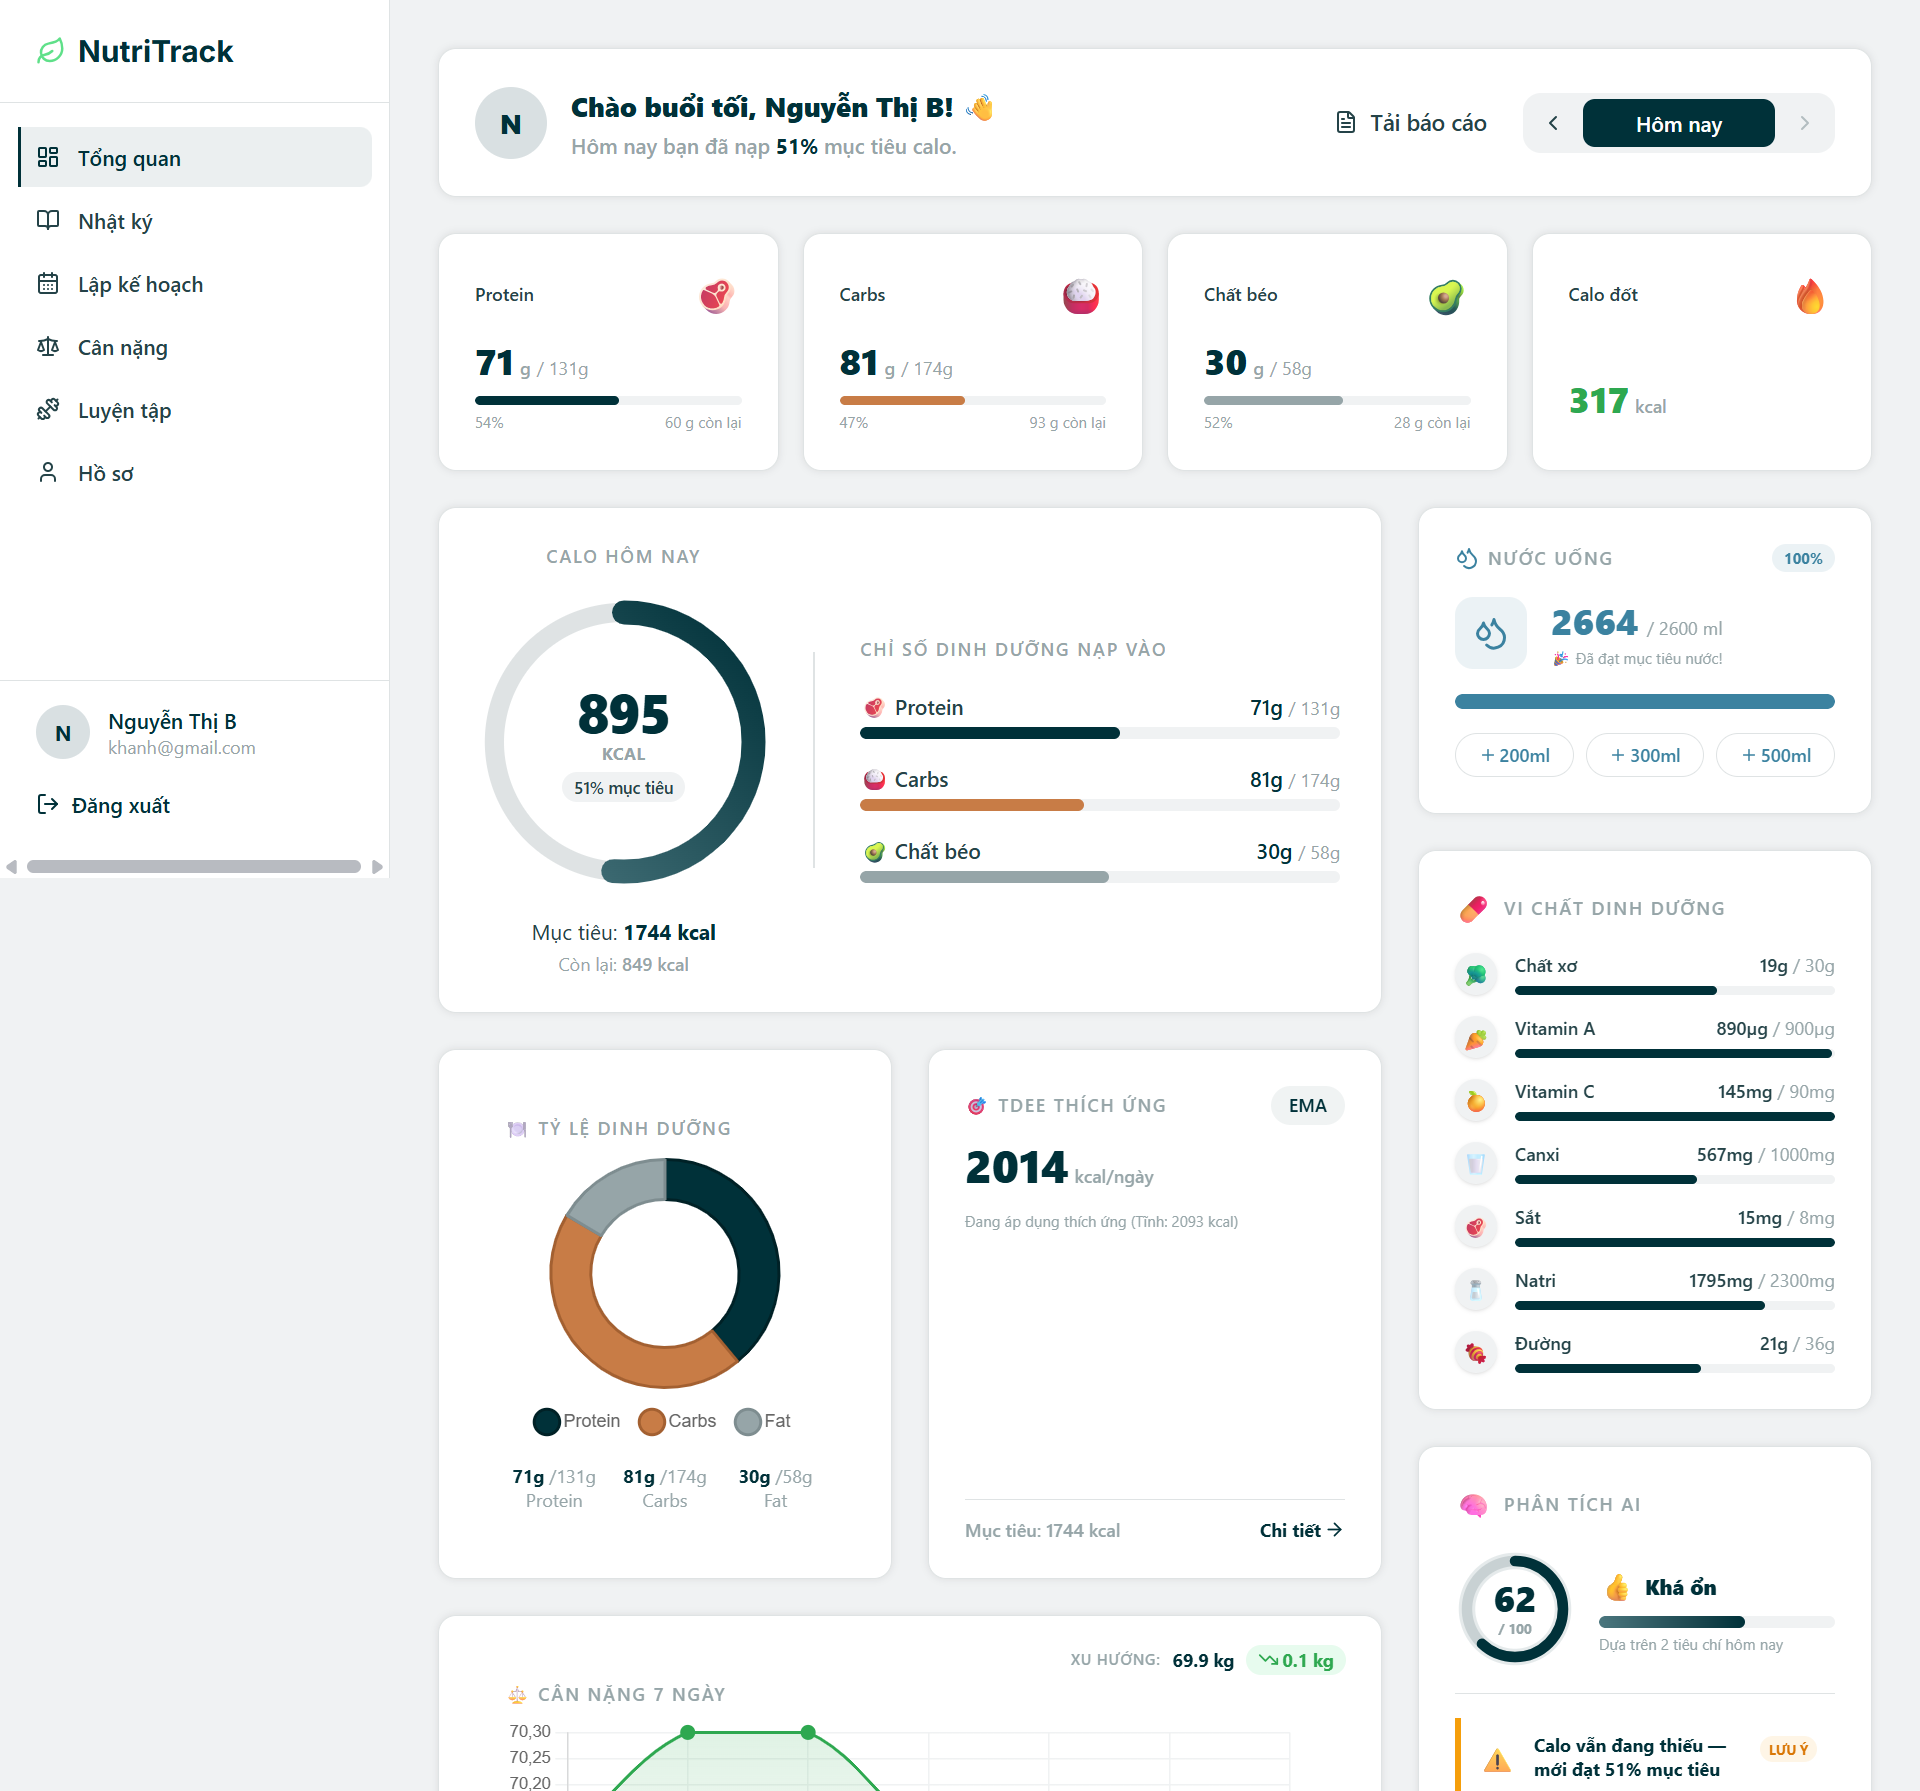
\includegraphics[height=5cm, width=\textwidth, keepaspectratio]{images/dashboard_overview_cropped.png} \\
            \vspace{0.2cm}
            \small \textbf{Dashboard}
        \end{column}
        \begin{column}{0.33\textwidth}
            \centering
            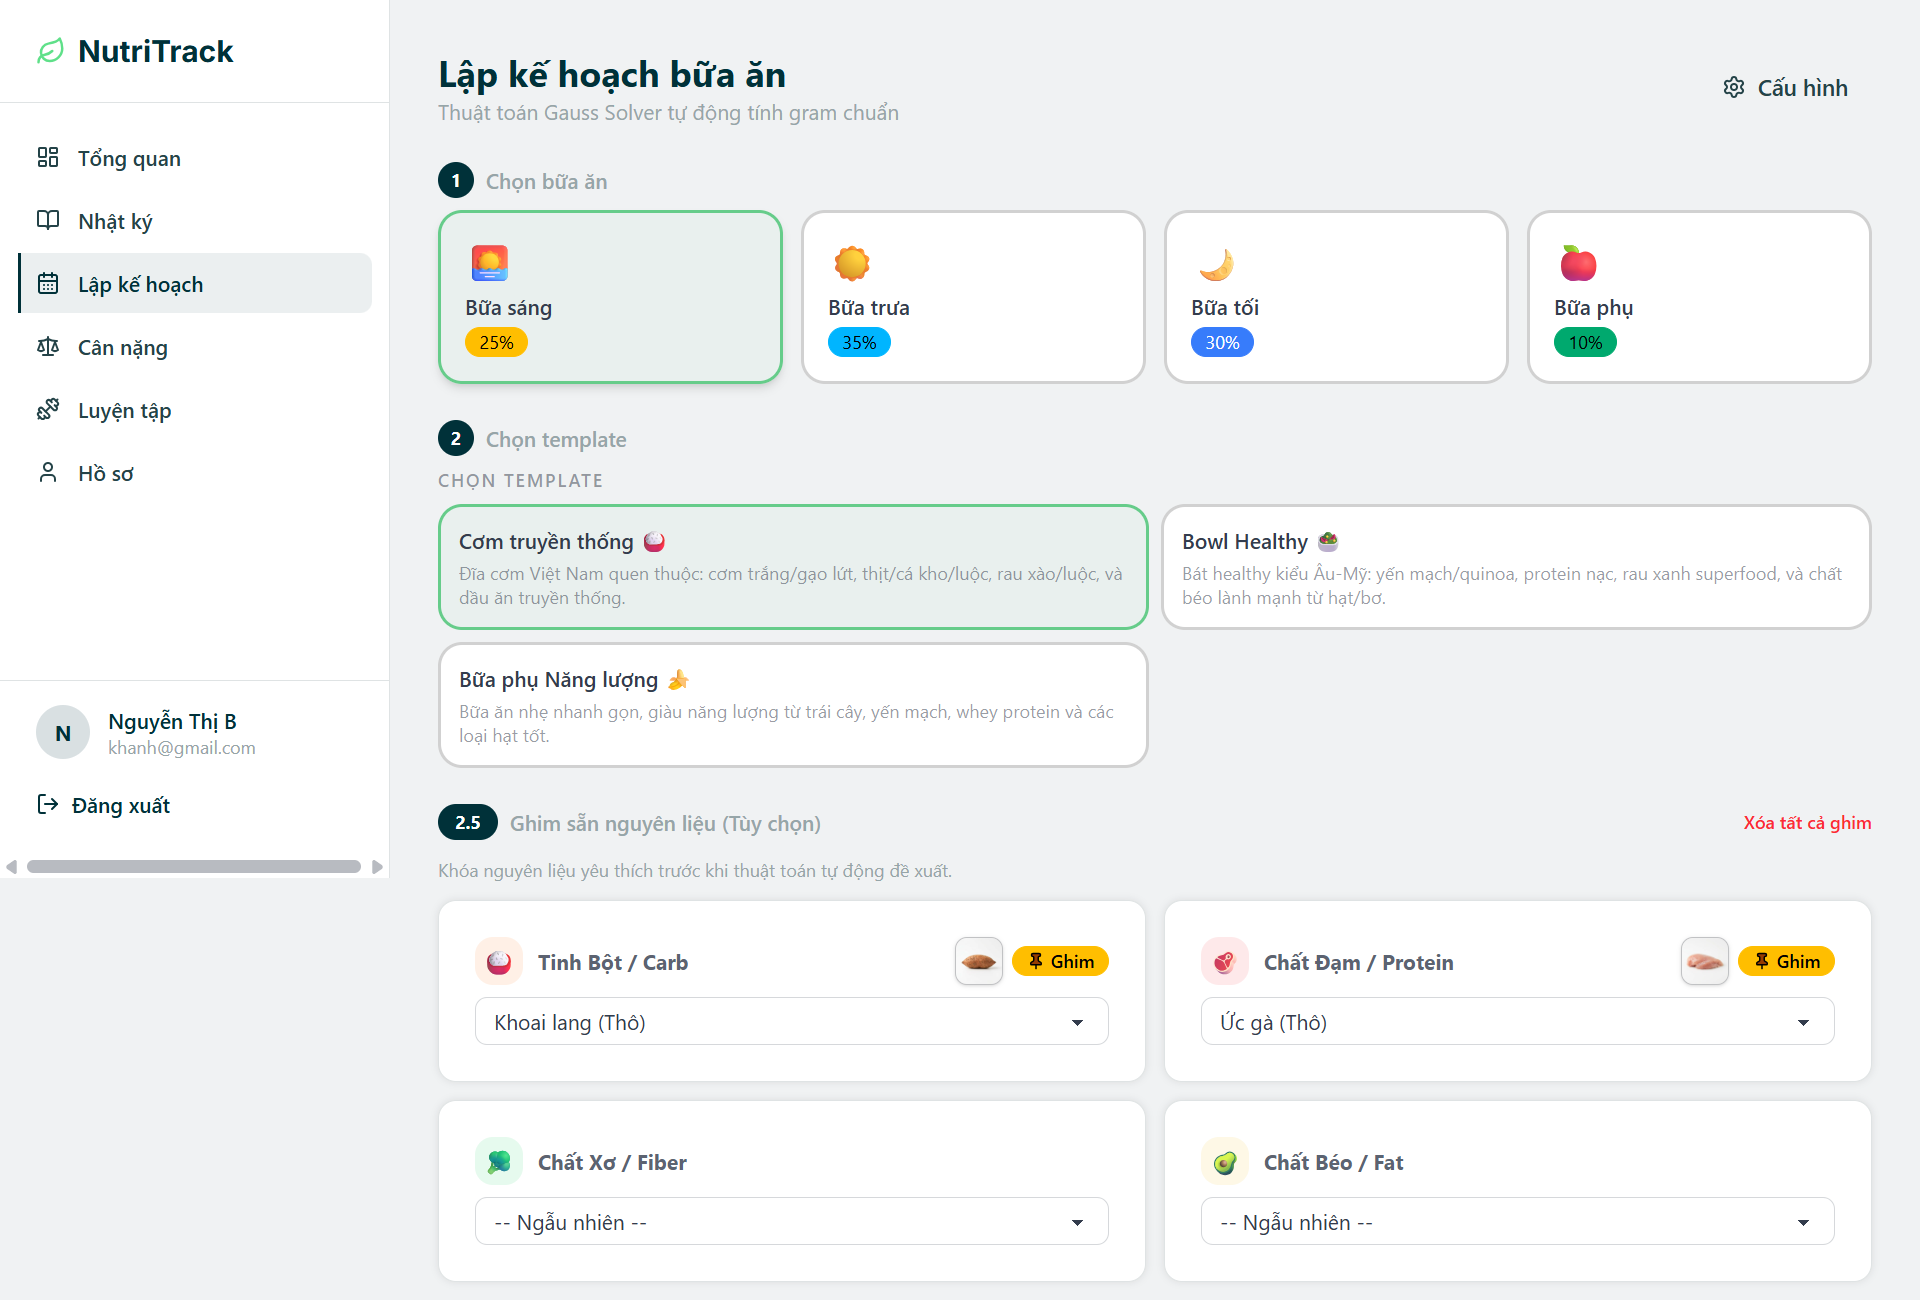
\includegraphics[height=5cm, width=\textwidth, keepaspectratio]{images/meal_planner_cropped.png} \\
            \vspace{0.2cm}
            \small \textbf{Meal Planner}
        \end{column}
        \begin{column}{0.33\textwidth}
            \centering
            
\includegraphics[height=5cm, width=\textwidth, keepaspectratio]{images/scanner_step1_cropped.png} \\
            \vspace{0.2cm}
            \small \textbf{Hybrid Scanner}
        \end{column}
    \end{columns}
\end{frame}

% Thời lượng dự kiến: 1 phút
\begin{frame}{Nền tảng tính toán dinh dưỡng (Nutrition Core)}
    \begin{itemize}
        \item \textbf{BMI \& BMR (Mifflin-St Jeor):} Đánh giá thể trạng và tính chuyển hóa cơ bản.
        \item \textbf{TDEE tĩnh:} $\text{BMR} \times \text{PAL}$ — ước tính tổng năng lượng tiêu hao theo hệ số hoạt động.
        \item \textbf{Phân bổ macro:} Protein / Carb / Fat theo mục tiêu. \textit{Khóa an toàn:} mục tiêu $\geq$ BMR.
    \end{itemize}
    
    \vspace{0.2cm}
    \begin{center}
    \begin{tikzpicture}[>=Stealth, node distance=0.8cm,
        steplabel/.style={rectangle, draw=NutriDark, fill=white, rounded corners, minimum height=0.6cm, text centered, font=\footnotesize},
        arrow/.style={->, thick, NutriDark}]
        
        \node[steplabel] (profile) {Hồ sơ cá nhân};
        \node[steplabel, right=of profile] (bmi) {BMI};
        \node[steplabel, right=of bmi] (bmr) {BMR};
        \node[steplabel, right=of bmr] (tdee) {TDEE};
        \node[steplabel, below=0.6cm of tdee] (goal) {Mục tiêu năng lượng};
        \node[steplabel, left=of goal, fill=NutriGreen!20] (dist) {\textbf{Phân bổ dinh dưỡng}};
        
        \draw[arrow] (profile) -- (bmi);
        \draw[arrow] (bmi) -- (bmr);
        \draw[arrow] (bmr) -- (tdee);
        \draw[arrow] (tdee) -- (goal);
        \draw[arrow] (goal) -- (dist);
    \end{tikzpicture}
    \end{center}
    
    \vspace{0.3cm}
    \centering\small \textit{TDEE tĩnh là \textbf{điểm khởi đầu} — slide tiếp theo sẽ trình bày cách hệ thống \textbf{hiệu chỉnh} giá trị này theo dữ liệu thực tế.}
\end{frame}

% Thời lượng dự kiến: 1 phút 30 giây
\begin{frame}{Adaptive TDEE – Điều chỉnh theo dữ liệu thực tế}
    \begin{center}
    \begin{tikzpicture}[>=Stealth, node distance=0.35cm and 0.4cm,
        box/.style={rectangle, draw=NutriDark, fill=white, rounded corners, minimum height=0.7cm, text width=3.5cm, text centered, font=\scriptsize},
        arrow/.style={->, thick, NutriDark}]
        
        \node[box] (n1) {Dữ liệu ăn uống + cân nặng theo tuần};
        \node[box, right=of n1] (n2) {Kiểm tra đủ dữ liệu\\[-0.3ex]\tiny $\ge 5$ ngày nhật ký, $\ge 2$ lần cân};
        \node[box, right=of n2] (n3) {Tính AvgIntake + EMA làm mượt cân nặng};
        
        \node[box, below=0.4cm of n3] (n4) {Suy ra TDEE ước tính của tuần};
        \node[box, left=of n4] (n5) {Giới hạn $\pm30\%$ quanh TDEE tĩnh};
        \node[box, left=of n5] (n6) {Trung bình trượt tối đa 4 tuần};
        
        \node[box, below=0.4cm of n5, minimum width=11.3cm, text width=11cm, fill=NutriGreen!20] (n7) {\textbf{Lưu lịch sử; đủ $\ge 2$ tuần hợp lệ mới cập nhật Adaptive TDEE}};
        
        \draw[arrow] (n1) -- (n2);
        \draw[arrow] (n2) -- (n3);
        \draw[arrow] (n3) -- (n4);
        \draw[arrow] (n4) -- (n5);
        \draw[arrow] (n5) -- (n6);
        \draw[arrow] (n6.south) -- (n6.south |- n7.north);
    \end{tikzpicture}
    \end{center}
    
    \vspace{0.1cm}
    \begin{center}
        \colorbox{NutriDark!10}{\textbf{Công thức: } $TDEE\_\text{ước\_tính} = \text{AvgIntake} - \left( \frac{\Delta\text{Weight} \times 7700}{7} \right)$} \\
        \vspace{0.15cm}
        \small \textit{\textcolor{NutriDark}{TDEE tĩnh là điểm khởi đầu; Adaptive TDEE hiệu chỉnh dần theo dữ liệu thực tế.}}
    \end{center}
    
    \vspace{0.1cm}
    \begin{columns}[T]
        \begin{column}{0.5\textwidth}
            \textcolor{NutriDark}{\textbf{\modulelabel{Thuật toán EMA (Lý thuyết gốc)}}}
            \begin{itemize}
                \item \scriptsize Công thức: $\text{EMA}_t = \alpha \cdot x_t + (1 - \alpha) \cdot \text{EMA}_{t-1}$
                \item \scriptsize $\alpha \in (0, 1)$: Hệ số làm mượt.
                \item \scriptsize $\alpha$ nhỏ $\rightarrow$ trọng số quá khứ lớn.
                \item \scriptsize Ưu điểm: Bộ nhớ $O(1)$, thời gian $O(n)$.
            \end{itemize}
        \end{column}
        \begin{column}{0.48\textwidth}
            \textcolor{NutriDark}{\textbf{\modulelabel{Áp dụng trong hệ thống}}}
            \begin{itemize}
                \item \scriptsize $\alpha = 0.1$: Ít bị ảnh hưởng bởi dao động ngày.
                \item \scriptsize Warm-up 14 ngày (khởi tạo EMA ổn định).
                \item \scriptsize Anti-smoothing kép: Dùng $\text{TDEE}_{\text{thô}}$ để tính.
                \item \scriptsize Confidence score: 7 ngày (High) $\rightarrow$ 5 ngày (Low).
            \end{itemize}
        \end{column}
    \end{columns}
\end{frame}

% Thời lượng dự kiến: 1 phút
\begin{frame}{Phân tích chất lượng dinh dưỡng}
    \begin{columns}[T]
        \begin{column}{0.52\textwidth}
            \modulelabel{Food Scoring}
            \vspace{0.2cm}
            
            \scriptsize
            \textbf{Ý tưởng:} Đánh giá mật độ dinh dưỡng trên 100 kcal.
            \vspace{0.1cm}
            \begin{itemize}
                \item Điểm cơ sở = \textbf{50} (thang 0--100).
                \item \textbf{Cộng điểm:} Protein $\geq 5$g/100kcal (+25), Fiber $\geq 1.25$g (+25).
                \item \textbf{Trừ điểm:} Sodium $> 150$mg/100kcal (−25), Sugar $> 5$g (−25).
                \item \textbf{Vi chất:} Vitamin A, C, Canxi, Sắt — bonus tối đa +10/vi chất.
                \item \textbf{Hard Cap:} Vi chất quá kém $\rightarrow$ trần 50; Thiếu xơ $\rightarrow$ trần 60.
            \end{itemize}
        \end{column}
        
        \begin{column}{0.44\textwidth}
            \modulelabel{Daily Health Score}
            \vspace{0.2cm}
            
            \scriptsize
            \textbf{Ý tưởng:} Đánh giá tổng thể 1 ngày ăn uống.
            \vspace{0.1cm}
            \begin{itemize}
                \item Tổng hợp dữ liệu nhật ký (calo, macro, nước) theo ngày.
                \item So sánh với mục tiêu cá nhân + RDI (Recommended Daily Intake).
                \item Phát hiện: vượt calo, thiếu protein, mất cân đối macro, thiếu nước.
                \item Ưu tiên cảnh báo theo mức độ nghiêm trọng.
                \item Điểm sức khỏe 0--100 (điểm phạt/thưởng + Hard Cap).
            \end{itemize}
        \end{column}
    \end{columns}
    
    \vspace{0.3cm}
    \centering
    \scriptsize \textit{*Các ngưỡng dinh dưỡng tham khảo FDA Daily Values (2000 kcal/ngày).}
\end{frame}

% Thời lượng dự kiến: 1 phút 30 giây
\begin{frame}{Meal Planner – Tính khẩu phần bằng phương pháp khử Gauss}
    \textbf{Bài toán:} Từ mục tiêu Protein, Carb và Fat của bữa ăn, hệ thống lựa chọn tổ hợp nguyên liệu phù hợp và tính khối lượng cần sử dụng.
    
    \vspace{0.3cm}
    \begin{columns}[T]
        \begin{column}{0.46\textwidth}
            \textbf{1. Mô hình $A\mathbf{x} = \mathbf{b}$} ($A$: ma trận macro, $\mathbf{x}$: k.lượng, $\mathbf{b}$: m.tiêu)
            \vspace{0.15cm}
            
            \textbf{2. Thuật toán Khử Gauss ($n=3$):}
            \begin{itemize}
                \item \scriptsize \textbf{Forward + Pivoting:} Đưa $A$ về tam giác trên, hoán vị dòng.
                \item \scriptsize \textbf{Back Sub:} Giải ngược tìm $\mathbf{x}$.
                \item \scriptsize Nếu $|pivot| < 10^{-10}$: Ma trận suy biến.
            \end{itemize}
            \vspace{0.15cm}
            
            \textbf{3. Xử lý ngoại lệ (Edge cases):}
            \begin{itemize}
                \item \scriptsize Nghiệm âm, $<10$g, $>500$g $\rightarrow$ Không khả thi.
                \item \scriptsize Retry tối đa 15 lần, lưu best-attempt.
            \end{itemize}
        \end{column}

        \begin{column}{0.53\textwidth}
            \begin{center}
            \begin{tikzpicture}[>=Stealth, node distance=0.32cm,
                box/.style={rectangle, draw=NutriDark, fill=white, rounded corners, minimum height=0.45cm, text centered, font=\scriptsize, align=center},
                arrow/.style={->, NutriDark}]
                \node[box] (n1) {Mục tiêu ngày + cấu hình bữa};
                \node[box, below=of n1] (n2) {Phân bổ mục tiêu từng bữa};
                \node[box, below=of n2] (n3) {Chọn nguyên liệu theo template};
                \node[box, below=of n3] (n4) {Rau/fiber: cố định 200 g, trừ macro};
                \node[box, below=of n4] (n5) {\textbf{Khử Gauss}\\[-0.3ex]\textbf{+ Partial Pivoting}};
                \node[box, below=of n5] (n6) {Kiểm tra nghiệm \& khối lượng};
                \node[box, below=of n6, fill=NutriGreen!20] (n7) {Hợp lệ $\rightarrow$ Meal Plan \\ Không hợp lệ $\rightarrow$ Retry $\le$ 15};
                
                \draw[arrow] (n1) -- (n2);
                \draw[arrow] (n2) -- (n3);
                \draw[arrow] (n3) -- (n4);
                \draw[arrow] (n4) -- (n5);
                \draw[arrow] (n5) -- (n6);
                \draw[arrow] (n6) -- (n7);
            \end{tikzpicture}
            \end{center}
        \end{column}
    \end{columns}
\end{frame}

% Thời lượng dự kiến: 1 phút 15 giây
% ─── HYBRID NUTRITION SCANNER SLIDE ───────────────────────────────────────
% Sơ đồ được chuyển đổi sang TikZ từ yêu cầu người dùng
% ─────────────────────────────────────────────────────────────────────────
\begin{frame}{Hybrid Nutrition Scanner}
    \textbf{Ưu tiên dữ liệu cục bộ trước, chỉ gọi nguồn bên ngoài khi cần.}
    \vspace{0.1cm}
    \begin{center}
    \resizebox{0.93\textwidth}{!}{
    \begin{tikzpicture}[>=Stealth, node distance=0.2cm and 0.8cm,
        box/.style={rectangle, draw=NutriDark, fill=white, rounded corners, minimum height=0.5cm, minimum width=3.6cm, text centered, font=\scriptsize, align=center},
        arrow/.style={->, thick, NutriDark}
    ]
    
    % Nhánh 1
    \node[box, fill=blue!10, draw=blue!60] (barcode) {\textbf{Quét Barcode}};
    \node[box, fill=yellow!20, draw=orange!60, below=0.3cm of barcode] (l1) {\textbf{Lớp 1:} Local DB Verified};
    \node[box, fill=yellow!20, draw=orange!60, below=0.2cm of l1] (l2) {\textbf{Lớp 2:} Local DB Unverified};
    \node[box, fill=yellow!20, draw=orange!60, below=0.2cm of l2] (l3) {\textbf{Lớp 3:} Open Food Facts};
    \node[box, fill=red!15, draw=red!60, below=0.2cm of l3] (l4) {\textbf{Lớp 4:} Cả 3 lớp không tìm thấy};
    
    % Hiển thị kết quả (của nhánh 1)
    \node[box, below=0.3cm of l4] (result) {\textbf{Hiển thị kết quả}};
    
    % Nhánh 2
    \node[box, fill=green!15, draw=green!60, right=2.4cm of barcode] (photo) {\textbf{Chụp ảnh nhãn dinh dưỡng}};
    \node[box, below=0.35cm of photo] (ai) {\textbf{Gemini AI Vision} \\ (Trích xuất dữ liệu từ ảnh)};
    \node[box, fill=yellow!20, draw=orange!60, below=0.35cm of ai] (physics) {\textbf{Kiểm tra tính hợp lý dữ liệu} \\ (Physics Validation)};
    \node[box, below=0.35cm of physics] (user) {\textbf{Người dùng} \\ kiểm tra \& xác nhận};
    
    % Lưu dữ liệu / Thêm vào nhật ký
    \path (result) -- (user) coordinate[midway] (mid);
    \node[box, fill=green!20, draw=NutriDark, minimum width=9cm, below=0.5cm of mid] (save) {\textbf{Lưu dữ liệu / Thêm vào nhật ký (Diary)}};
    
    % Background layers
    \begin{scope}[on background layer]
        \coordinate (barcode_top) at ([yshift=0.35cm]barcode.north);
        \coordinate (l1ext) at ([xshift=1.4cm]l1.east);
        \node[rectangle, draw=blue!30, fill=blue!5, rounded corners, inner sep=0.25cm, fit=(barcode_top) (l4) (result) (l1ext)] (bg1) {};
        \node[anchor=north west, font=\scriptsize\bfseries, text=blue!80!black] at ([yshift=-4pt, xshift=4pt]bg1.north west) {Nhánh 1 — Tra cứu Barcode};
        
        \coordinate (photo_top) at ([yshift=0.35cm]photo.north);
        \node[rectangle, draw=green!30, fill=green!5, rounded corners, inner sep=0.25cm, fit=(photo_top) (user)] (bg2) {};
        \node[anchor=north west, font=\scriptsize\bfseries, text=green!80!black] at ([yshift=-4pt, xshift=4pt]bg2.north west) {Nhánh 2 — AI Vision};
    \end{scope}
    
    % To make labels match the background
    \tikzset{lbl1/.style={font=\tiny, fill=blue!5, inner sep=1pt}}
    
    % Arrows Nhánh 1
    \draw[arrow, blue!60] (barcode) -- (l1);
    \draw[arrow, blue!60] (l1) -- node[lbl1] {Không đạt} (l2);
    \draw[arrow, blue!60] (l2) -- node[lbl1] {Không đạt} (l3);
    \draw[arrow, blue!60] (l3) -- node[lbl1] {Không đạt} (l4);
    
    \draw[->, thick, blue!60] (l1.east) -- ++(1.2,0) node[lbl1, pos=0.5] {Đạt} |- ([yshift=4pt]result.east);
    \draw[->, thick, blue!60] (l2.east) -- ++(0.9,0) node[lbl1, pos=0.5] {Đạt} |- (result.east);
    \draw[->, thick, blue!60] (l3.east) -- ++(0.6,0) node[lbl1, pos=0.5] {Đạt} |- ([yshift=-4pt]result.east);
    
    % Arrows Nhánh 2
    \draw[arrow, green!60!black] (photo) -- (ai);
    \draw[arrow, green!60!black] (ai) -- (physics);
    \draw[arrow, green!60!black] (physics) -- (user);
    
    % The red arrow from Lớp 4 to Chụp ảnh
    \draw[->, thick, red!70!black] (l4.east) -- ++(1.5,0) |- (photo.west);
    
    % Arrows to Save
    \draw[arrow] (result.south) -- (result.south |- save.north);
    \draw[arrow] (user.south) -- (user.south |- save.north);
    
    \end{tikzpicture}
    }
    \end{center}
\end{frame}


% Thời lượng dự kiến: 50 giây
\begin{frame}{Kết quả thực nghiệm và kiểm thử}
    \begin{columns}[T]
        \begin{column}{0.33\textwidth}
            \modulelabel{Chức năng chính}
            \vspace{0.2cm}
            
            \small \textbf{8 module} chức năng hoạt động end-to-end.
        \end{column}
        
        \begin{column}{0.33\textwidth}
            \modulelabel{Xử lý dữ liệu}
            \vspace{0.2cm}
            
            \small \textbf{4 thuật toán} chuyên biệt (Gauss, EMA, Food Scoring, Health Score).
        \end{column}
        
        \begin{column}{0.33\textwidth}
            \modulelabel{Kiến trúc kỹ thuật}
            \vspace{0.2cm}
            
            \small \textbf{40+ API endpoint}, Cron Job tự động hàng tuần.
        \end{column}
    \end{columns}
    
    \vspace{0.5cm}
    \begin{center}
        \small
        \renewcommand{\arraystretch}{1.3}
        \begin{tabularx}{0.98\textwidth}{>{\hsize=0.28\hsize}X | >{\hsize=0.72\hsize}X}
            \toprule
            \textbf{Nhóm kiểm thử} & \textbf{Kết quả} \\
            \midrule
            Khử Gauss (Meal Planner) & Giải hệ 3×3; phát hiện ma trận suy biến ($|pivot| < 10^{-10}$); retry tối đa 15 lần, lưu best-attempt. \\
            Adaptive TDEE & Test 7 ngày: TDEE tĩnh 2500 $\rightarrow$ Adaptive 2200 kcal (−12\%); phát hiện plateau, đề xuất giảm mục tiêu. \\
            Scanner API / AI Vision & Tra cứu Barcode qua 3 lớp fallback; AI Vision trích xuất + Physics Validation kiểm tra tính hợp lý. \\
            \bottomrule
        \end{tabularx}
    \end{center}
\end{frame}

% Thời lượng dự kiến: 20-30 giây
\begin{frame}{Kịch bản demo}
    \begin{center}
    \begin{tikzpicture}[>=Stealth, 
        node distance=0.8cm,
        steplabel/.style={rectangle, draw=NutriDark, fill=white, rounded corners, minimum height=0.8cm, text width=2.5cm, text centered, font=\footnotesize},
        arrow/.style={->, thick, NutriDark}]
        
        \node[steplabel, fill=NutriGreen!20] (s1) {1. Dashboard \& Hồ sơ tổng quan};
        \node[steplabel, right=of s1] (s2) {2. Ghi nhận bữa ăn \& quan sát};
        \node[steplabel, right=of s2] (s3) {3. Demo Meal Planner hoặc Scanner};
        \node[steplabel, right=of s3] (s4) {4. Xem nhanh Adaptive TDEE};
        
        \draw[arrow] (s1) -- (s2);
        \draw[arrow] (s2) -- (s3);
        \draw[arrow] (s3) -- (s4);
    \end{tikzpicture}
    \end{center}
    
    \vspace{1cm}
    \centering
    \Large \textit{Tiến hành demo trực tiếp trên hệ thống...}
\end{frame}

% Thời lượng dự kiến: 50 giây
\begin{frame}{Kết luận và hướng phát triển}
    \begin{columns}[T]
        \begin{column}{0.48\textwidth}
            \modulelabel{Kết quả đạt được}
            \vspace{0.2cm}
            \begin{itemize}
                \small \setlength{\itemsep}{2pt}
                \item Xây dựng hệ thống web quản lý dinh dưỡng với đầy đủ chức năng đề ra.
                \item Tích hợp theo dõi dinh dưỡng, cân nặng, nước uống và luyện tập.
                \item Triển khai thuật toán Adaptive TDEE, Food Scoring và Meal Planner.
                \item Xây dựng kiến trúc Client–Server giao tiếp qua RESTful API.
                \item Xuất báo cáo PDF tổng hợp, tích hợp phân tích Adaptive TDEE.
            \end{itemize}
        \end{column}
        
        \begin{column}{0.48\textwidth}
            \modulelabel{Hướng phát triển}
            \vspace{0.2cm}
            \begin{itemize}
                \small \setlength{\itemsep}{2pt}
                \item Mở rộng cơ sở dữ liệu thực phẩm nội bộ.
                \item Kiểm thử với nhiều người dùng và dữ liệu dài hạn.
                \item Tiếp tục đánh giá thuật toán Adaptive TDEE.
                \item Cải thiện độ tin cậy của Hybrid Scanner và dữ liệu đầu vào.
            \end{itemize}
        \end{column}
    \end{columns}
    
    \vspace{0.3cm}
    \centering
    \Large \textbf{\textcolor{NutriDark}{Em xin chân thành cảm ơn thầy cô đã lắng nghe!}} \\
    \vspace{0.2cm}
    \normalsize \textit{Q\&A}
\end{frame}

\end{document}
